\documentclass{report}
\usepackage{graphicx}
\graphicspath{{./images/}}
\usepackage{geometry}
\usepackage{hyperref}
\usepackage{paralist}
\usepackage[round]{natbib}
\usepackage{sectsty}
\usepackage{gensymb}
\usepackage{caption}
\usepackage{subcaption}
\usepackage{listings}
\usepackage[space]{grffile}
\usepackage{latexsym}
\usepackage{amsfonts,amsmath,amssymb}
\usepackage{url}
\usepackage{hyperref}
\hypersetup{colorlinks=false,pdfborder={0 0 0}}
\usepackage{textcomp}
\usepackage{longtable}
\usepackage{multirow,booktabs}
\newcommand{\truncateit}[1]{\truncate{0.8\textwidth}{#1}}
\newcommand{\scititle}[1]{\title[\truncateit{#1}]{#1}} 
\usepackage[parfill]{parskip}
\usepackage[inline]{enumitem}
\usepackage{fixltx2e}
\usepackage[super]{nth}
\usepackage[final]{pdfpages}

% Typeface
\usepackage{ifxetex}
\ifxetex
  \usepackage{fontspec}
  \defaultfontfeatures{Ligatures=TeX} % To support LaTeX quoting style
  \setmainfont[Mapping=tex-text, Color=textcolor]{HelveticaNeue}
  %\setmainfont[Mapping=tex-text, Color=textcolor]{Avenir LT Std}
\else
  \usepackage[T1]{fontenc} 
  \usepackage[utf8]{inputenc}
  \renewcommand{\familydefault}{\sfdefault}
  \usepackage{helvet}
\fi
\chapterfont{\Large} % \sffamily

% Title page
\usepackage{xcolor}
\definecolor{titlepagecolor}{cmyk}{0,0,0,0}
\definecolor{namecolor}{cmyk}{0,0,0,1} 
\definecolor{chaptertitlepagecolor}{cmyk}{0,0,0,0.9}
\definecolor{chapternamecolor}{cmyk}{0,0,0,0.3}  

\begin{document}

%---------------------------------------------- TITLE ----------------------------------------------


\includepdf[pages={-}]{examtitlepage.pdf}


%---------------------------------------------- CONTENTS ----------------------------------------------

\tableofcontents

\pagebreak



%---------------------------------------------- CHAPTERS ----------------------------------------------

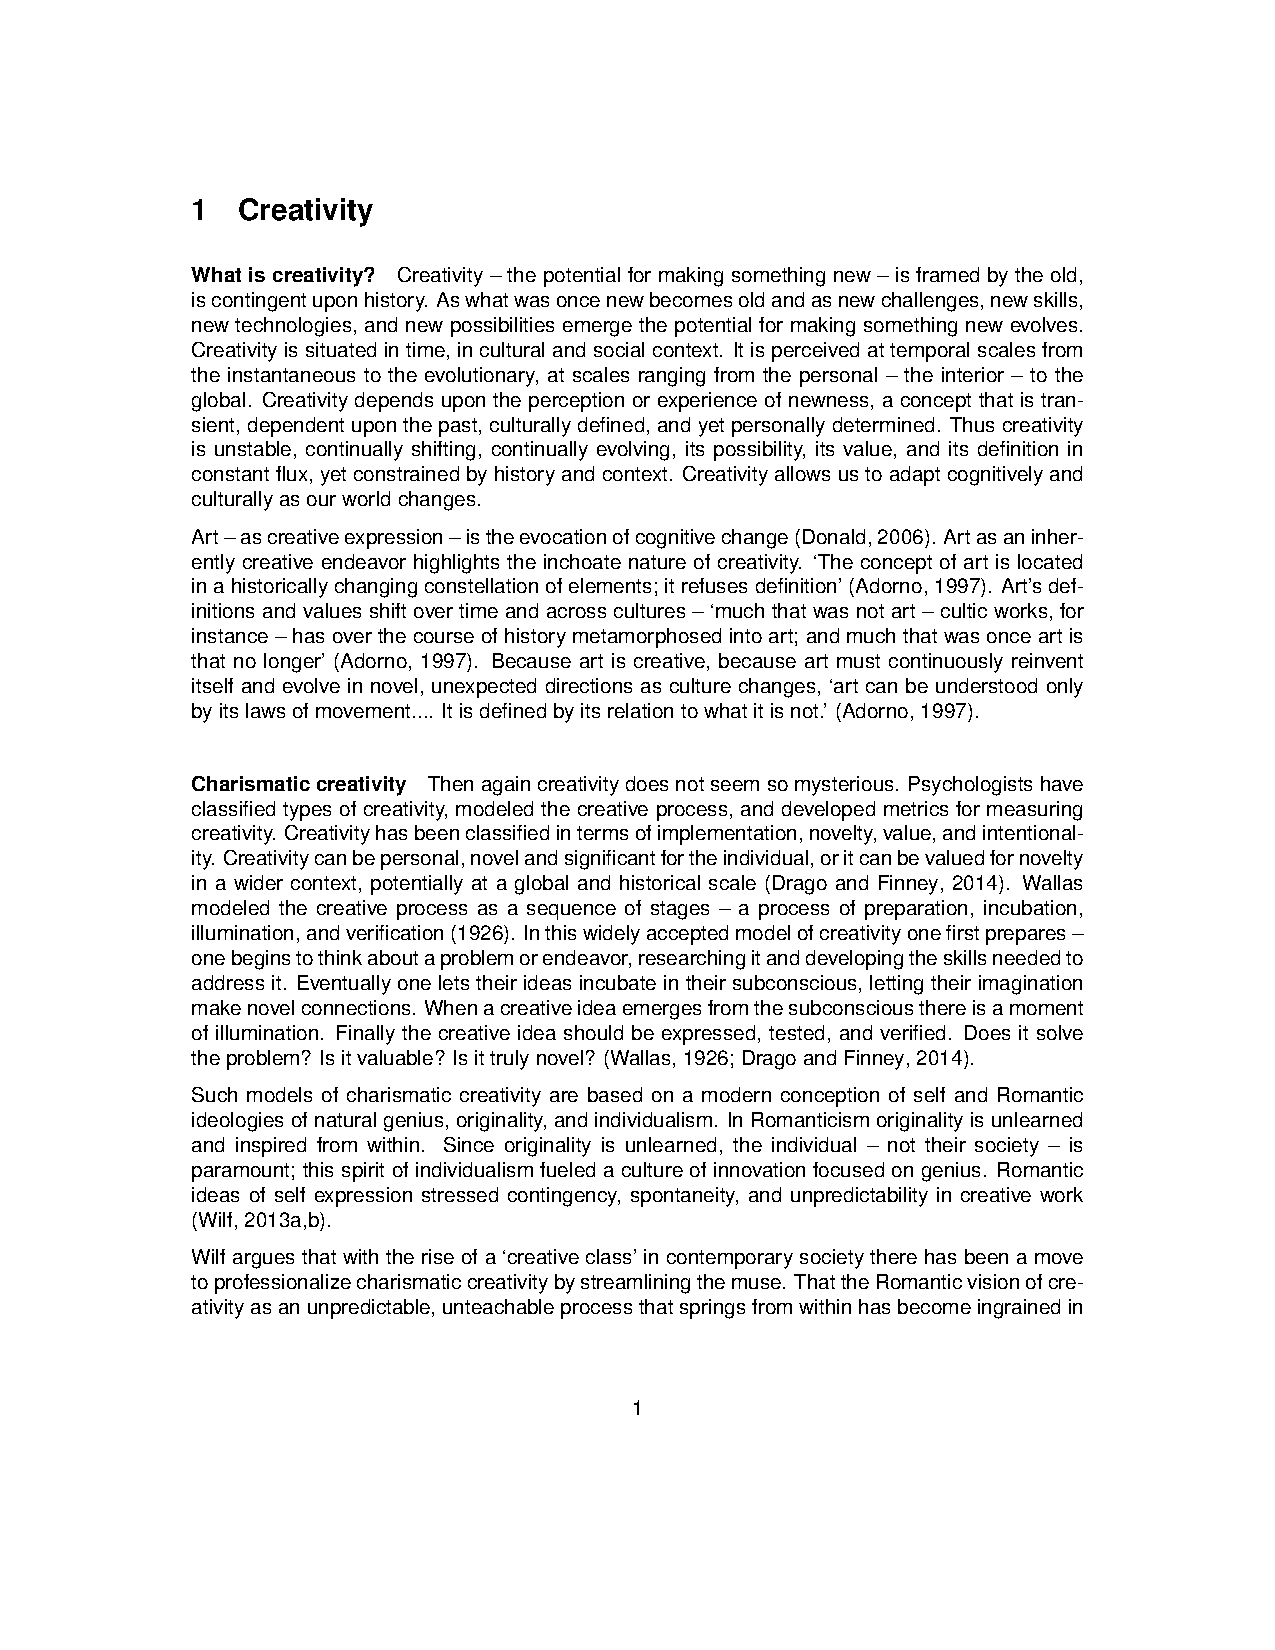
\includepdf[pages={-}, addtotoc={1, chapter, 1, Creativity, creativity}]{creativity.pdf}

\includepdf[pages={-}, addtotoc={1, chapter, 1, Engagement, engagement}]{engagement.pdf}

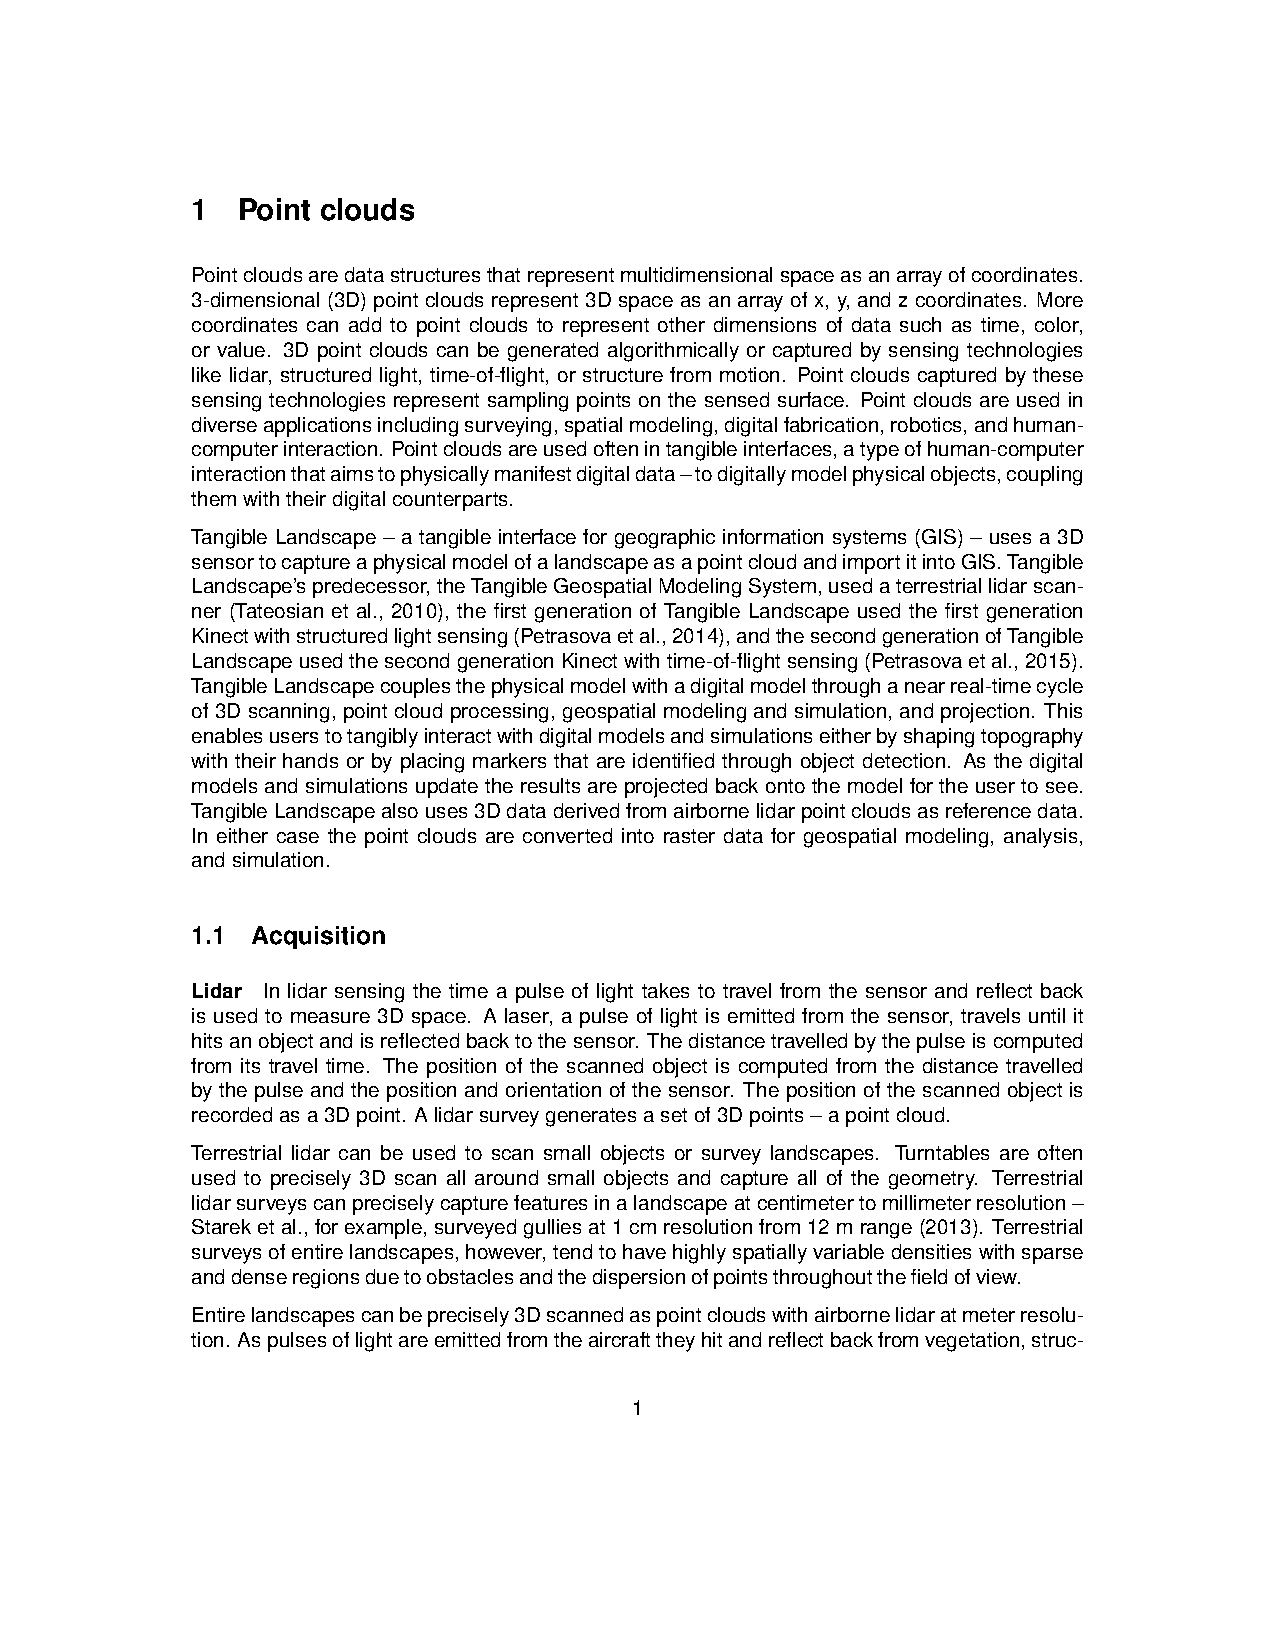
\includepdf[pages={-}, addtotoc={1, chapter, 1, Point Clouds, point_clouds}]{point_clouds.pdf}

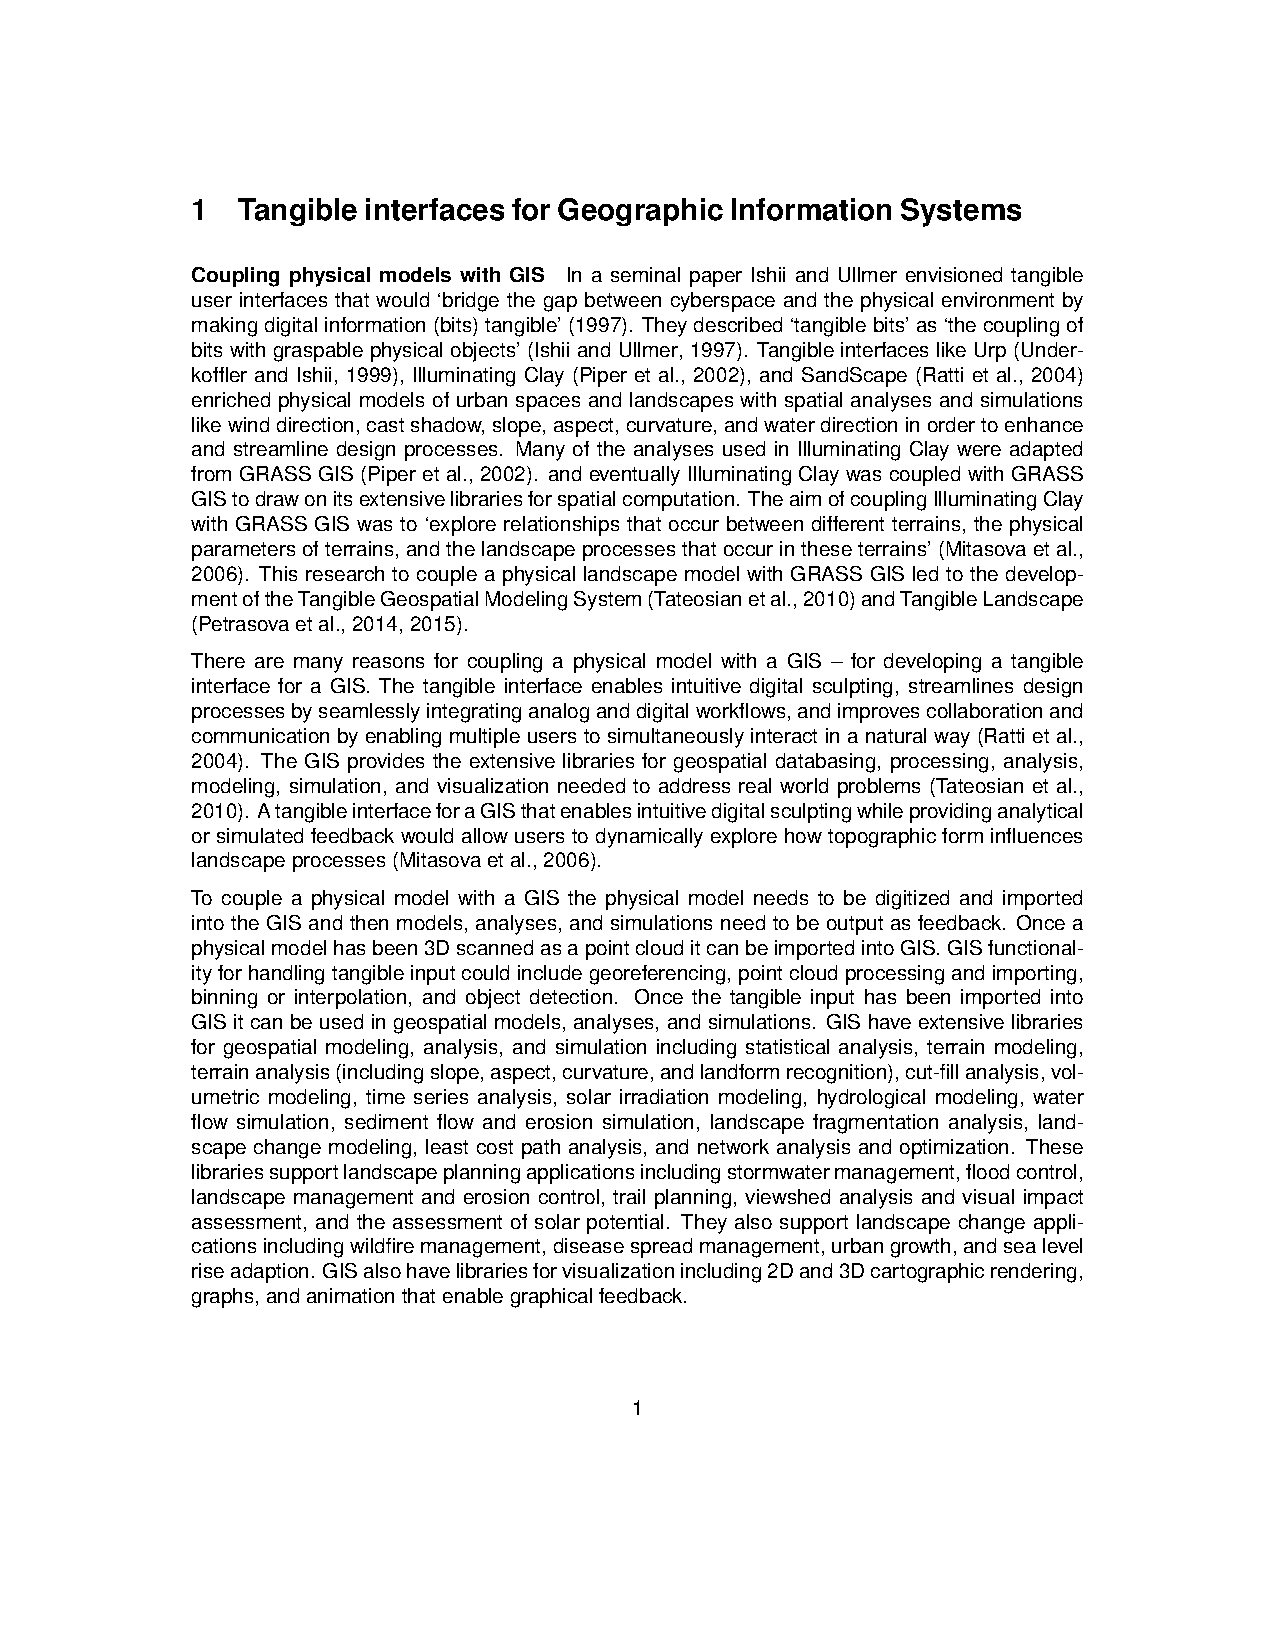
\includepdf[pages={-}, addtotoc={1, chapter, 1, Tangible interfaces for GIS, tangible_gis}]{tangible_gis.pdf}


%---------------------------------------------- BIBLIOGRAPHY ----------------------------------------------

\bibliographystyle{plainnat}
\bibliography{tangible_topography} 
\end{document}

